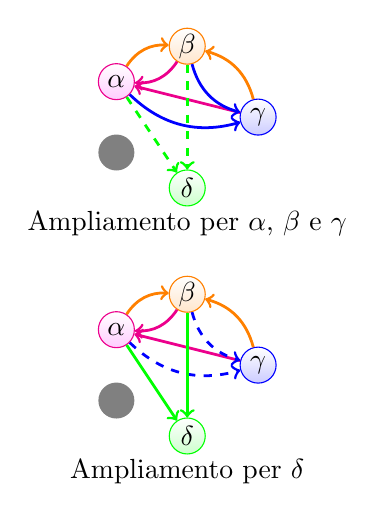
\begin{tikzpicture}[scale=.45]

\tikzset{mynode/.style={circle,minimum size=13pt,inner sep=0pt,draw, top color=white ,bottom color=blue!20, blue,text=black},}
\tikzset{mynode2/.style={circle,minimum size=13pt,inner sep=0pt,draw, top color=white ,bottom color=magenta!20, magenta,text=black},}
\tikzset{mynode3/.style={circle,minimum size=13pt,inner sep=0pt,draw, top color=white ,bottom color=orange!20, orange,text=black},}
\tikzset{mynode6/.style={circle,minimum size=13pt,inner sep=0pt,draw, top color=white ,bottom color=green!20, green,text=black},}
\tikzset{mynode7/.style={circle,fill=gray,minimum size=13pt,inner sep=0pt,},draw}
\tikzset{label/.style={minimum size=15pt,inner sep=0pt,},}


%PENTAGONO  
\draw (0,0) node [mynode7] () {};
\draw (0,2) node [mynode2] (alfa1) {$\alpha$};
\draw (4,1) node [mynode] (gamma1) {$\gamma$};
\draw (2,-1) node [mynode6] (delta1) {$\delta$};
\draw (2,3) node [mynode3] (beta1) {$\beta$};

\draw[->,magenta,line width=1pt] (beta1) to[bend left](alfa1);
\draw[->,magenta,line width=1pt] (gamma1) -- (alfa1);
\draw[->,orange,line width=1pt] (alfa1) to[bend left](beta1);
\draw[->,orange,line width=1pt] (gamma1)to[bend right](beta1);
\draw[->,blue,line width=1pt] (alfa1) to[bend right] (gamma1);
\draw[->,blue,line width=1pt](beta1)to[bend right]  (gamma1);    
\draw[->,green,dashed,line width=1pt] (alfa1) -- (delta1);
\draw[->,green,dashed,line width=1pt](beta1) -- (delta1);     
\draw(2,-2) node[label] (l) {Ampliamento per $\alpha$, $\beta$ e $\gamma$};
  

%PENTAGONO2  
\draw (0,-7) node [mynode7] () {};
\draw (0,-5) node [mynode2] (alfa2) {$\alpha$};
\draw (4,-6) node [mynode] (gamma2) {$\gamma$};
\draw (2,-8) node [mynode6] (delta2) {$\delta$};
\draw (2,-4) node [mynode3] (beta2) {$\beta$};

\draw[->,magenta,line width=1pt] (beta2) to[bend left](alfa2);
\draw[->,magenta,line width=1pt] (gamma2) -- (alfa2);
\draw[->,orange,line width=1pt] (alfa2) to[bend left](beta2);
\draw[->,orange,line width=1pt] (gamma2)to[bend right](beta2);
\draw[->,blue,dashed,line width=1pt] (alfa2) to[bend right] (gamma2);
\draw[->,blue,dashed,line width=1pt](beta2) to[bend right] (gamma2);    
\draw[->,green,line width=1pt] (alfa2) -- (delta2);
\draw[->,green,line width=1pt](beta2) -- (delta2);     
\draw(2,-9) node[label] (l) {Ampliamento per $\delta$};
     
 
 
     
\end{tikzpicture}